\documentclass[12pt]{article}

% 頁面設置
\usepackage[right=20mm, bottom=30mm, left=20mm]{geometry} % 頁面邊界
% \usepackage{multicol} % 頁面分欄
% \setlength{\columnsep}{1pt} % 欄間距
\usepackage{float} % 浮動物件 (圖表 H)

% 字體設定
\usepackage{type1cm} % 設定字體大小
\usepackage{xeCJK} % 中文字體
\def \nosystemfont {} % 關閉系統字型

% \setCJKmainfont{Noto Sans TC}
\ifdefined\nosystemfont
  \setCJKmainfont[
    Path=../font/,
    UprightFont={kaiu.ttf},
  ]{標楷體}
\else
  \setCJKmainfont{標楷體} % 標楷體
\fi

% 設定首行縮排
\newlength{\fullwidthspace}
\setlength{\fullwidthspace}{2em}  % 定義兩個全形空白的長度為2em
\setlength{\parindent}{\fullwidthspace}  % 設定段落首行縮排為兩個全形空白

\setlength{\parskip}{4pt} % 設定段落間距

% 套件區
\usepackage{enumitem} % 列表 (enumerate, itemize)
\usepackage{array} % 表格
\usepackage{makecell} % 表格換行

\usepackage{adjustbox}

\usepackage{longtable} % 長表格
\usepackage{indentfirst} % 自動首行縮排
\usepackage{fancyhdr} % 頁首頁尾
\usepackage{lastpage} % 最後一頁的頁數
\renewcommand{\arraystretch}{1.45} % 表格行高
\usepackage{collcell}
\usepackage{colortbl} % 表格顏色
\usepackage{xcolor} % 表格顏色
\usepackage{hhline} % 表格雙線
\usepackage{multirow} % 表格合併儲存格
\usepackage{multicol} % 表格合併儲存格
\usepackage{etoolbox} % 用 gappto 累積一個指令
\usepackage{keyval} % 參數的 key-value 對
\usepackage{amssymb} % 數學符號

\usepackage{graphicx} % 圖片
\usepackage{caption} % 圖片標題
\usepackage{subcaption} % 圖片子標題
\usepackage{subfloat} % 子圖片
\captionsetup[figure]{name={圖},labelsep=period}
\captionsetup[table]{name={表},labelsep=period}
\captionsetup{justification=centering} % 圖表置中

% 使用 hyperref 並設定
\usepackage[unicode=true,pdfusetitle,
 bookmarks=true,bookmarksnumbered=false,bookmarksopen=false,
 breaklinks=false,pdfborder={0 0 0},backref=true,colorlinks=false]
 {hyperref}

% \usepackage{amssymb} % 數學符號
% \usepackage[fleqn]{amsmath} % 數學排版, fleqn 選項讓數學式靠左對齊
\usepackage{tikz} % 繪圖
\usepackage{pgfplots} % 圖表
\usepgfplotslibrary{groupplots} % Group 圖表
% \usepackage{subfig} % 圖表子圖

\usepackage{footnote}
\usepackage{tablefootnote}

% tikz 設定
% \tikzset{every state, accepting/.style={double distance=2pt}}
% \usetikzlibrary{automata, positioning, arrows}
\usetikzlibrary{shapes,arrows,positioning}
\tikzstyle{startstop} = [rectangle, rounded corners, minimum width=3cm, minimum height=1cm,text centered, draw=black, fill=red!30]
\tikzstyle{process} = [rectangle, minimum width=3cm, minimum height=1cm, text centered, draw=black, fill=orange!30]
\tikzstyle{arrow} = [thick,->,>=stealth]

% fancyhdr 設定
\pagestyle{fancy}
\renewcommand{\footnotesize}{\normalsize} % 設定腳註字型大小
\renewcommand{\headrulewidth}{0pt} % 不要有頁首橫線
\renewcommand{\footrulewidth}{0pt} % 不要有頁尾橫線
\renewcommand{\contentsname}{\centering 目錄} % 目錄名稱
\renewcommand{\listfigurename}{\centering 圖目錄} % 圖目錄名稱
\renewcommand{\listtablename}{\centering 表目錄} % 表格目錄名稱
\renewcommand{\refname}{\centering 參考文獻} % 參考文獻名稱
\renewcommand{\appendixname}{\centering 附件} % 附件名稱
\lhead{}
\chead{Template Title}
\rhead{}
\lfoot{}
\cfoot{}
% \rfoot{ 共 \pageref{LastPage} 頁 第 \thepage 頁} 
\rfoot{第 \thepage 頁}

% \input{autolabel.tex}

\begin{document}

% 標題
\title{Template Title\\
  \vspace{0.5cm}
  \large Template Subtitle}
% \author{}
\date{}

% 封面
\maketitle % 標題
\begin{figure}[H]
  \centering
  
\includegraphics[width=0.3\textwidth]{images/LOGO.png}
\end{figure}
\begin{center}
  \vspace{1cm}
  \textbf{團隊名稱:普羅程式} \\
  \vspace{1cm}
  \textbf{指導老師:何立德、馬尚彬} \\
  \vspace{1cm}
  \textbf{學生姓名:簡蔚驊、林一、王裕傑} \\
\end{center}
\thispagestyle{empty} % 取消頁碼
\newpage

% 摘要
% \pagenumbering{roman}
\addcontentsline{toc}{section}{摘要}
\begin{center}
  \section*{摘要}
\end{center}

在台灣,資訊科技領域備受關注。110年智慧學習軟體系統的產值已達316億元,且每年有數百萬名國高中學生參與程式課程,形成龐大的市場需求。

普羅程式致力於改善程式教育環境,為教育者提供技術支援與教學工具的開發。普羅程式曾在全國性的創業競賽中獲得前四名、專題競賽中獲得特優。並擁有曾在IEEE研討會上發表AI方面論文,以及曾具備全端工程師專業背景的成員。

普羅程式的產品ProgLearn程式教學系統,以程式教師為中心設計,旨在使程式教學更加容易,並解決工具使用困難、師生間互動不即時的挑戰。ProgLearn是一個整合性教學平台,適用於多種場景,如線上課程、個人教師、學校課程、程式才藝班、補教業以及偏鄉教育。提供0延遲直播、課程與作業管理,以及具有即時反饋功能的數位儀表板、講義視覺化編輯、智慧引導和自動批改等多功能。

相對於其他教學平台與工具,ProgLearn更注重師生間的互動和即時狀況反饋,協助教師提高教學品質。同時,透過智慧、自動化的功能,有效降低教師的教學負擔。以推動聯合國永續發展目標中的優質教育,並致力於縮減城鄉教育差距。
\\ \par \noindent
% 關鍵字
\textbf{關鍵詞:}程式教學、數位學習、教學工具、教育科技、普羅程式
\thispagestyle{empty}
\newpage

% 所有目錄
\tableofcontents % 目錄
\addcontentsline{toc}{section}{目錄} 
\thispagestyle{empty}
\newpage

% \listoffigures % 圖目錄
% \addcontentsline{toc}{section}{圖目錄} 
% \thispagestyle{empty}
% \newpage

% \listoftables % 表目錄
% \addcontentsline{toc}{section}{表目錄} 
% \thispagestyle{empty}
% \newpage

% 參考文獻
% \addcontentsline{toc}{section}{參考文獻} 
% \pagenumbering{roman}
% \setcounter{page}{6}
% \begin{thebibliography}{99}
  \bibitem{ref:111產業產值調查報告} 數位發展部 數位產業署、財團法人資訊工業策進會。"111年台灣智慧學習產業產值調查報告 - 智慧學習產業整合輸出計畫",民111年。
  \bibitem{ref:110產業產值調查報告} 張筱祺、鐘映庭。"經濟部工業局110年度專案計畫 - 智慧學習產業整合輸出計畫全球輸出網絡佈建分項計畫 - 智慧學習產業產值調查報告。" 財團法人資訊工業策進會產業情報所委託研究報告。資訊工業策進會數位教育研究所,民110年。
  \bibitem{ref:學生數量} 政府資料公開平台(民113年1月16日)。全臺灣各級學校之學生數及畢業生數資料。民113年2月14日,取自:https://data.gov.tw/dataset/31436。
  \bibitem{ref:企業培訓} 陳旻萃。"智慧培訓模式的發展趨勢與應用。" 人事月刊,民105年6月6日,第370期。
  \bibitem{ref:老師的困難} 林文瑛、陳衍宏、周蔚倫。"新冠疫情下線上同步教學演練的啟示:課堂參與程度與課堂環境及學習經驗之關係。" 長庚人文社會學報,14:2(2021),179-214。
  \bibitem{ref:補教業者} 楊文君(2019年9月6日)。程式設計納入正式課綱 家教時薪達2000元以上。取自:https://www.rti.org.tw/news/view/id/2033475
  \bibitem{ref:家教} 秦宛萱(2019年9月7日)。抓住父母望子成龍的心!5成4學生想當家教 程式設計時薪高達2500元。取自:https://www.cmmedia.com.tw/home/articles/17410
\end{thebibliography} 
% \newpage

% 附件
% \addcontentsline{toc}{section}{附件} 
% \appendix
% \section{\centering 附件}

\subsection{產品功能展示}
\label{fig:Appendix-Product}
\begin{figure}[H]
	\begin{subfigure}{0.5\linewidth}
	  \centering
	  %   \href{https://raw.githubusercontent.com/programingtw/proglearn-plan/main/img/list.png}{ 
	  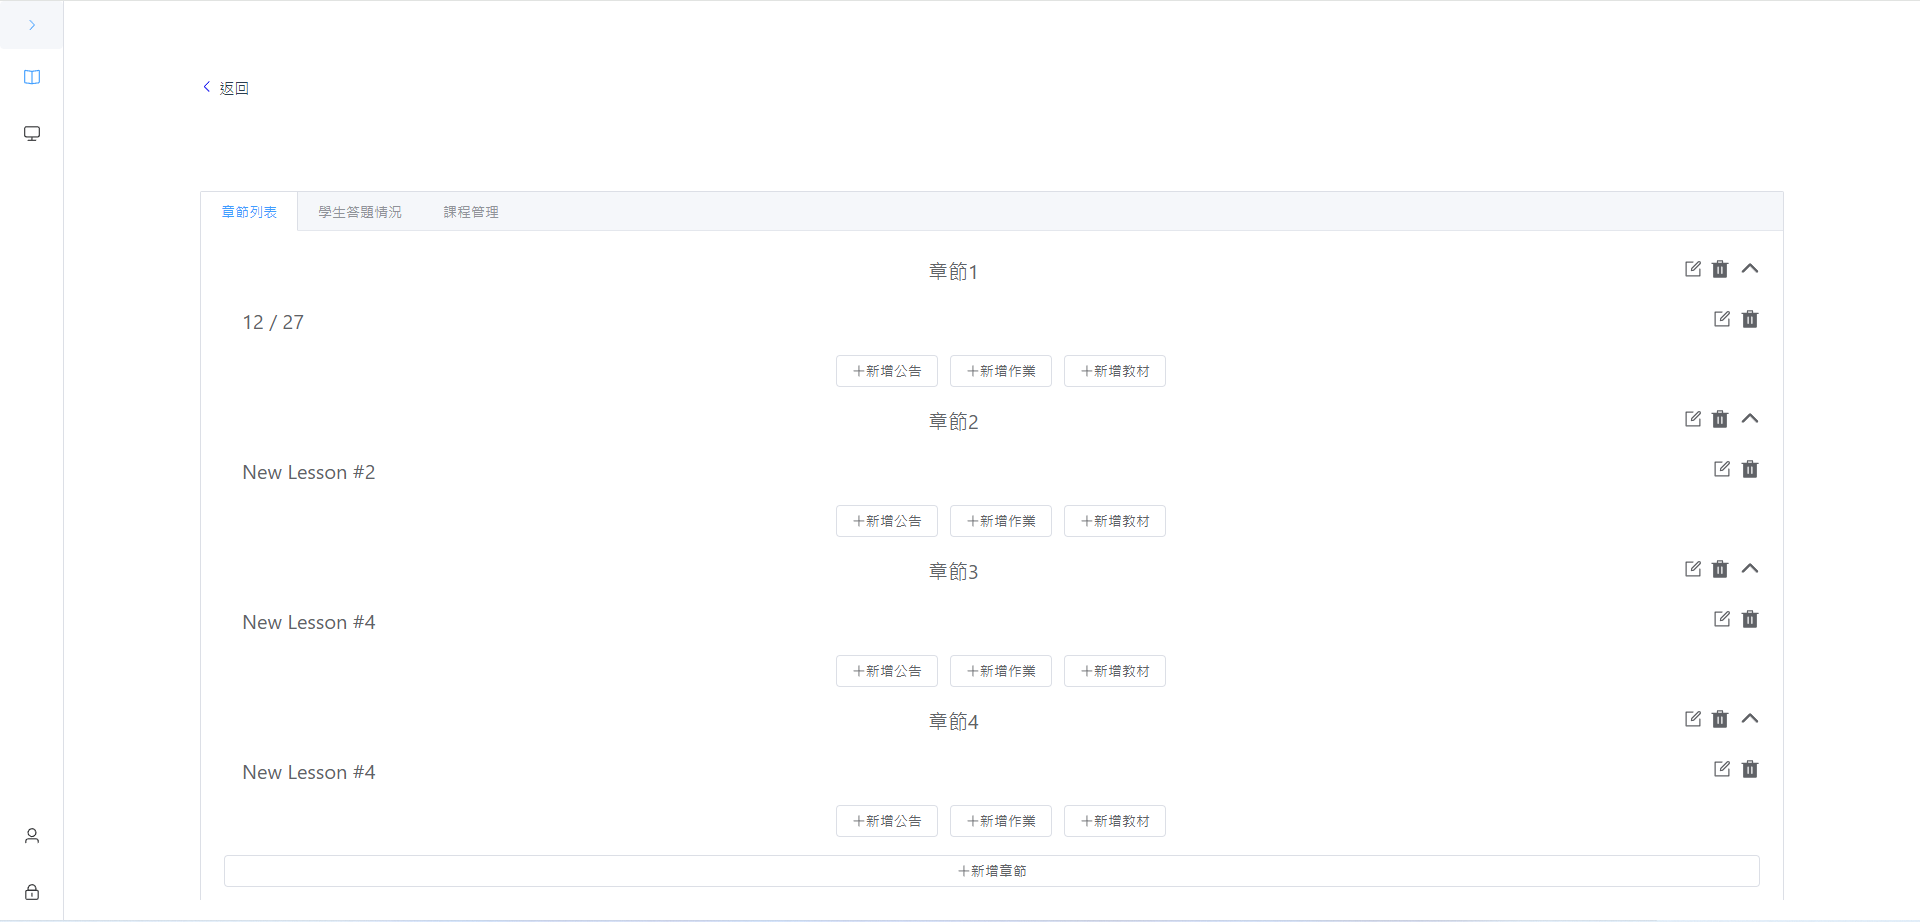
\includegraphics[width=0.75\textwidth]{images/chapter.png}
	  %   }
	  \caption{課程章節}
	\end{subfigure}
	\begin{subfigure}{0.5\linewidth}
	  \centering
	  %   \href{https://raw.githubusercontent.com/programingtw/proglearn-plan/main/img/course.png}{ 
	  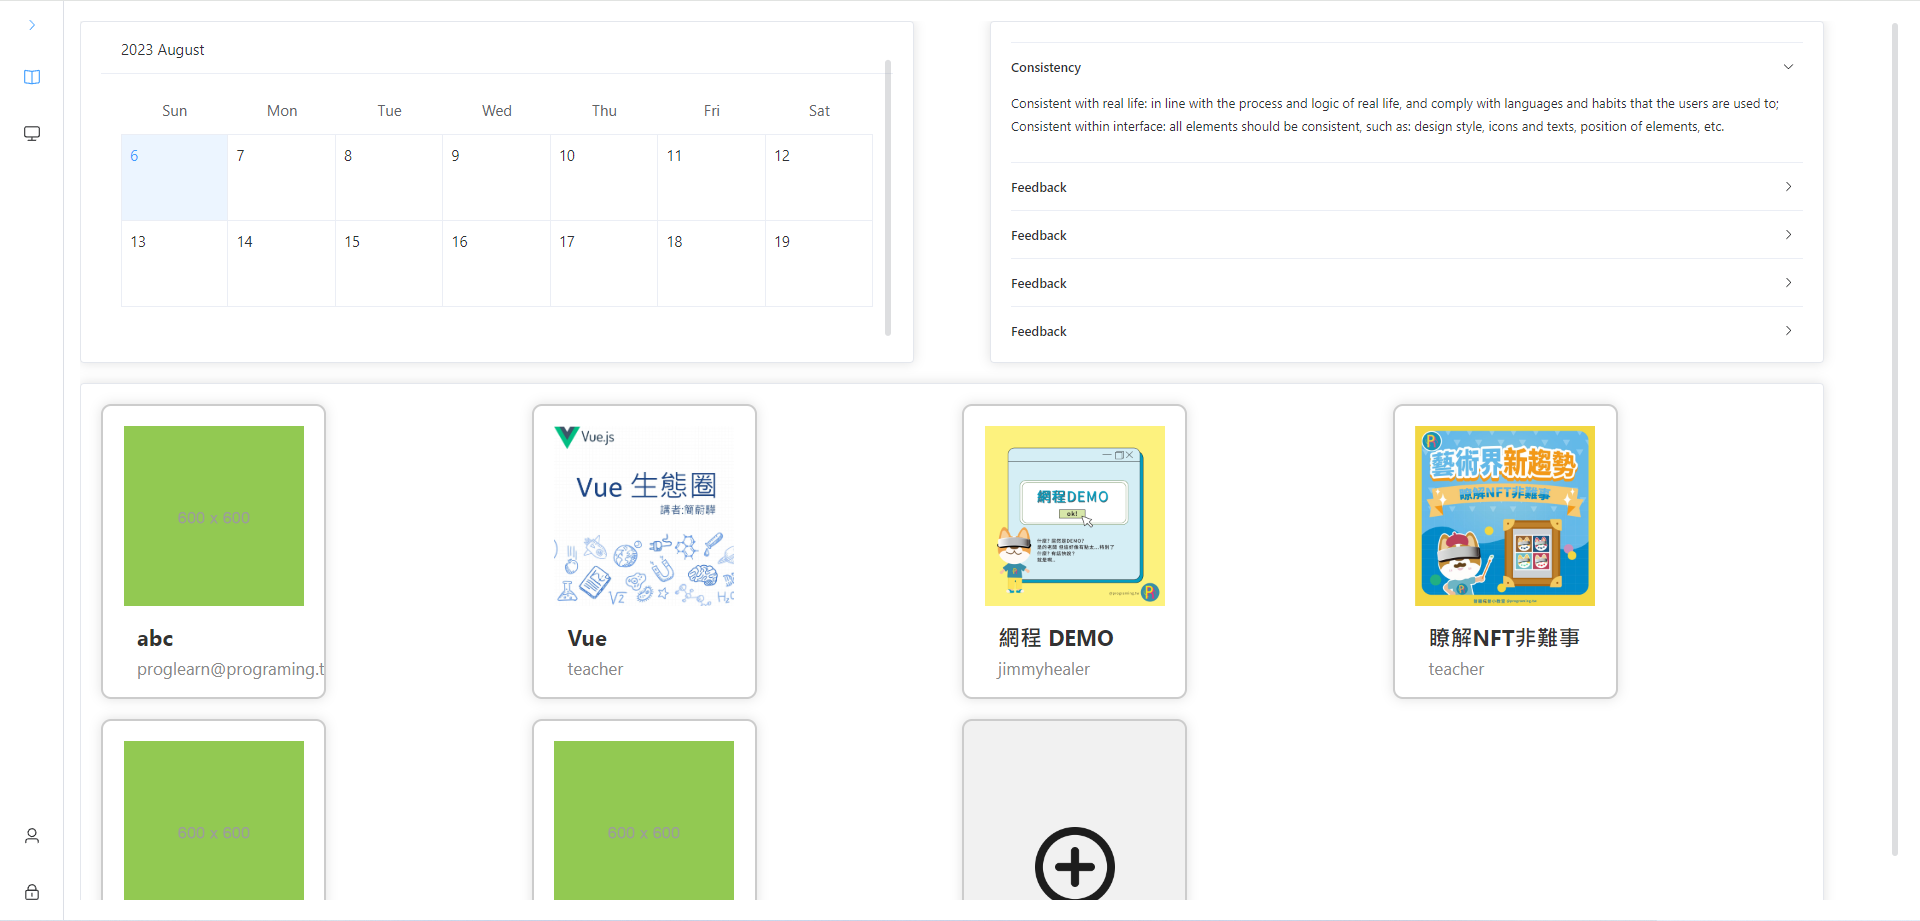
\includegraphics[width=0.75\textwidth]{images/course.png}
	  %   }
	  \caption{課程清單}
	\end{subfigure}
	\caption{課程相關頁面}
	\label{fig:course}
  \end{figure}
  
  \begin{figure}[H]
	\begin{subfigure}{0.5\linewidth}
	  \centering
	  %   \href{https://raw.githubusercontent.com/programingtw/proglearn-plan/main/img/list.png}{ 
	  
\includegraphics[width=0.75\textwidth]{images/homework.png}
	  %   }
	  \caption{作業作答}
	\end{subfigure}
	\begin{subfigure}{0.5\linewidth}
	  \centering
	  %   \href{https://raw.githubusercontent.com/programingtw/proglearn-plan/main/img/course.png}{ 
	  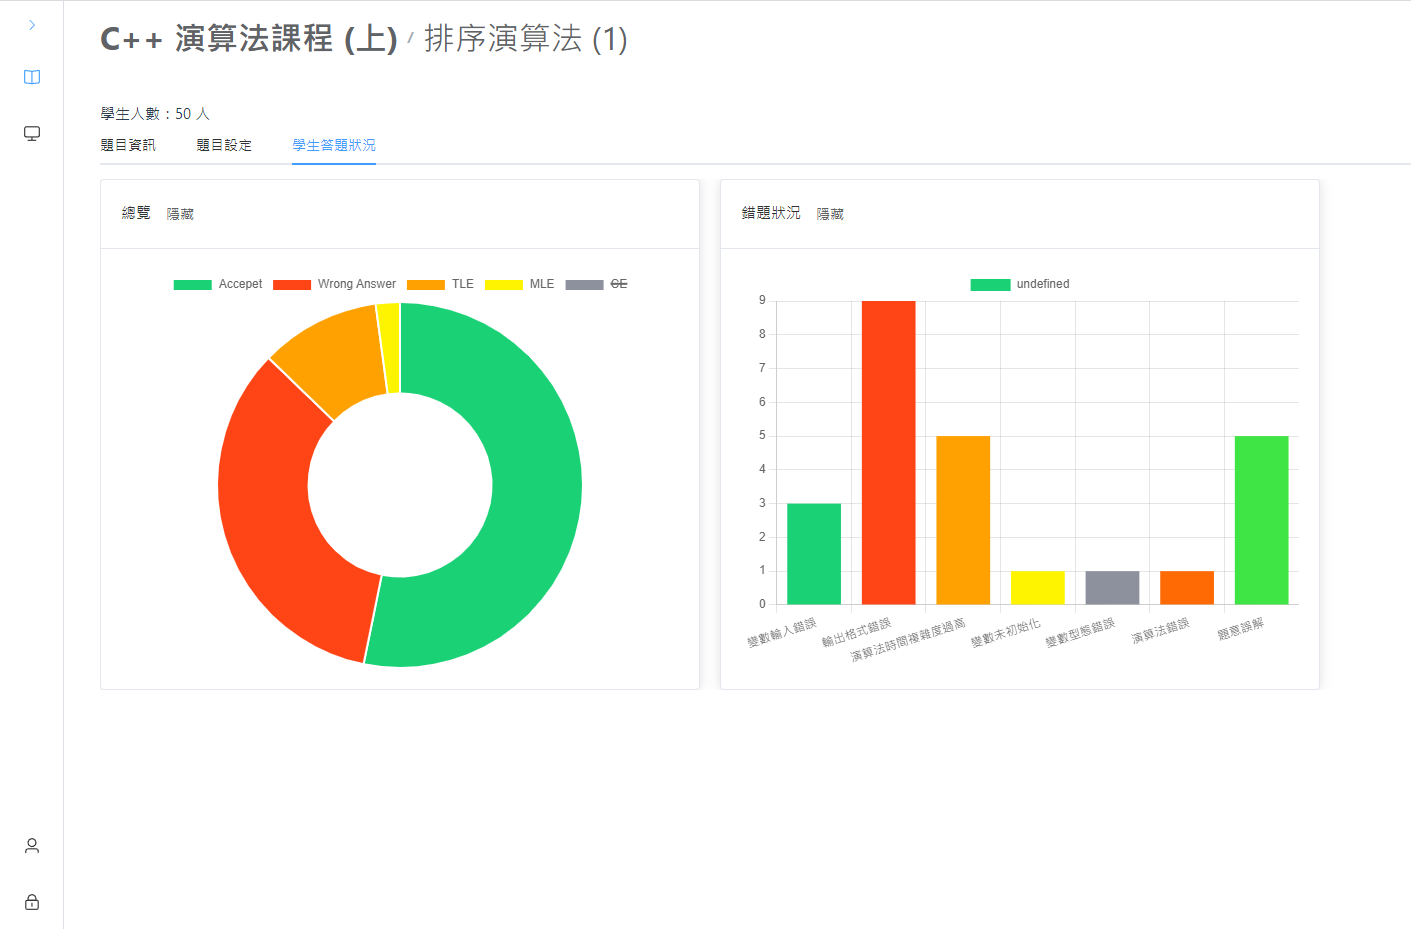
\includegraphics[width=0.75\textwidth]{images/feedback.png}
	  %   }
	  \caption{作業反饋}
	\end{subfigure}
	\caption{作業相關頁面}
	\label{fig:homework}
\end{figure}

\subsection{各平台教師數量}
\label{fig:Appendix-Teacher}
% 三張圖
\begin{figure}[H]
	\centering
	\begin{subfigure}{0.32\linewidth}
		\centering
		
\includegraphics[width=1\textwidth]{images/A-9007.png}
		\caption{AmazingTalker線上家教平台}
		\label{fig:Teacher-1}
	\end{subfigure}
	\begin{subfigure}{0.32\linewidth}
		\centering
		
\includegraphics[width=1\textwidth]{images/1111-2482.png}
		\caption{1111家教網}
		\label{fig:Teacher-2}
	\end{subfigure}
	\begin{subfigure}{0.32\linewidth}
		\centering
		
\includegraphics[width=1\textwidth]{images/pro360-2026.png}
		\caption{PRO360達人網}
		\label{fig:Teacher-3}
	\end{subfigure}
	\caption[各平台教師數量]{各平台教師數量\\(資料來源:於2024年2月22日,截取自AmazingTalker、1111家教網及PRO360達人網)}
\end{figure}

\subsection{線上教學平台分潤比例}
\label{fig:Appendix-profit-sharing}
% 兩張圖
\begin{figure}[H]
	\centering
	\begin{subfigure}{0.45\linewidth}
		\centering
		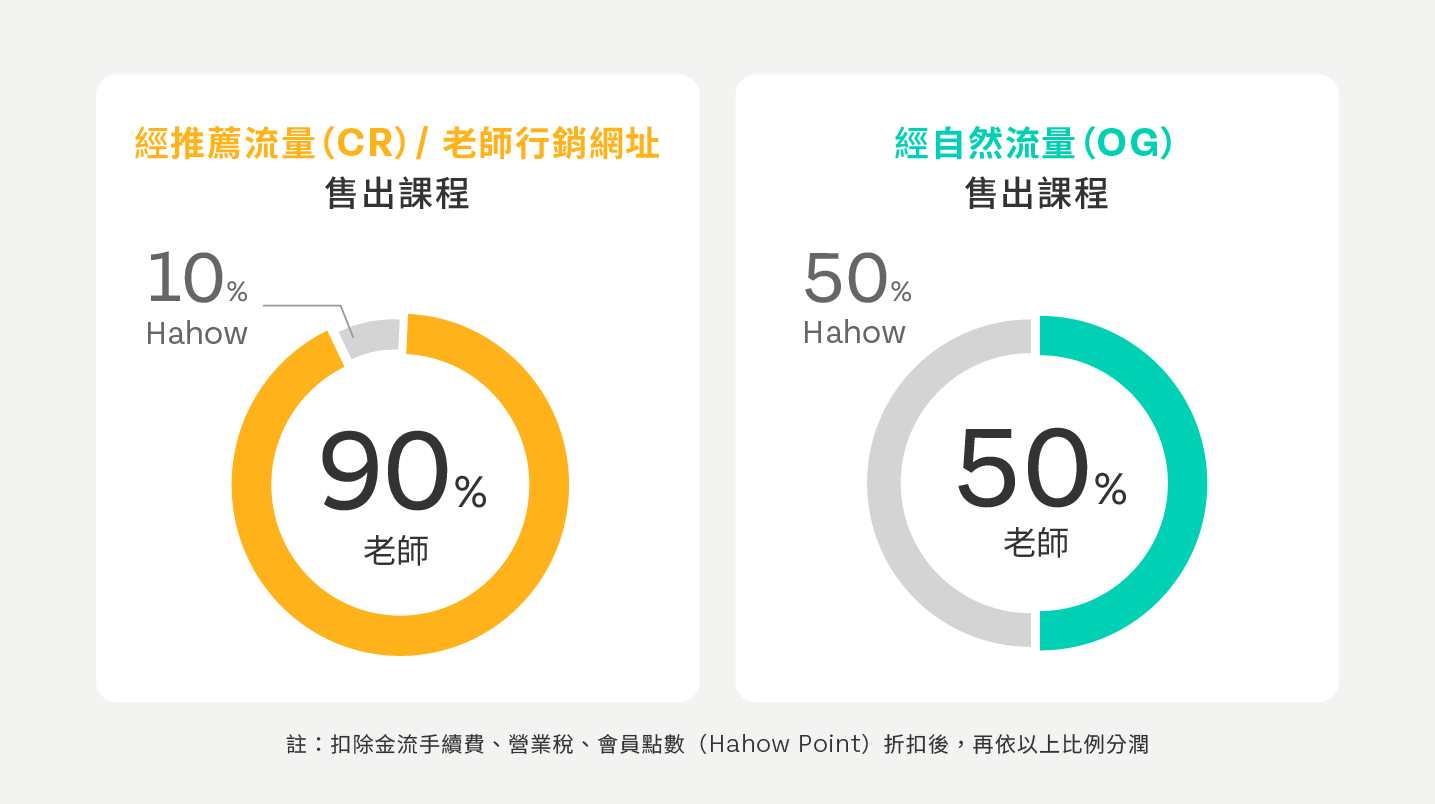
\includegraphics[width=1\textwidth]{images/hahow.png}
		\caption{Hahow好學校}
		\label{fig:Hahow}
	\end{subfigure}
	\begin{subfigure}{0.45\linewidth}
		\centering
		
\includegraphics[width=0.6\textwidth]{images/hiskio.png}
		\caption{HiSKIO 專業線上教學平台}
		\label{fig:HiSKIO}
	\end{subfigure}
	\caption[線上教學平台分潤比例]{線上教學平台分潤比例\\(資料來源:於2024年2月22日,截取自Hahow好學校及HiSKIO 專業線上教學平台)}
\end{figure}

\subsection{過去的行銷成果}
\label{fig:Appendix-Marketing}
\begin{figure}[H]
	\centering
	\begin{subfigure}{0.32\linewidth}
		\centering
		
\includegraphics[width=1\textwidth]{images/FB.png}
		\caption{Facebook}
		\label{fig:FB}
	\end{subfigure}
	\begin{subfigure}{0.32\linewidth}
		\centering
		
\includegraphics[width=0.6\textwidth]{images/IG.jpg}
		\caption{Instagram}
		\label{fig:IG}
	\end{subfigure}
	\begin{subfigure}{0.32\linewidth}
		\centering
		
\includegraphics[width=1\textwidth]{images/website.png}
		\caption{普羅官網}
		\label{fig:website}
	\end{subfigure}
	\caption[社群平台]{社群平台\\(資料來源:於2024年1月15日,截取自普羅Facebook、Instagram及官網)}
	\label{fig:platform}
\end{figure}

\begin{enumerate}
	\item Facebook:https://www.facebook.com/programing.edu.tw
	\item Instagram:https://www.instagram.com/programing.tw/
	\item 普羅官網:https://www.programing.tw/
\end{enumerate}

\subsection{過去的募資經驗}
\label{fig:Appendix-fundraising}
\begin{figure}[H]
	\centering
	
\includegraphics[width=0.8\textwidth]{images/flyingv-19600.png}
	\caption{flyingV群眾募資 - 成果}
	\label{fig:flyingv}
\end{figure}

\subsection{過去的創業研習經驗}
\label{fig:Appendix-Training}
\begin{figure}[H]
  \centering
  \begin{subfigure}{0.32\linewidth}
    \centering
    
\includegraphics[width=0.8\textwidth]{images/training-1.png}
    \caption{112 學年第一學期學生創業戰鬥營 - 林一}
    \label{fig:Training-1}
  \end{subfigure}
  \begin{subfigure}{0.32\linewidth}
    \centering
    
\includegraphics[width=0.8\textwidth]{images/training-2.png}
    \caption{112 學年第一學期學生創業新手村 - 簡蔚驊}
    \label{fig:Training-2}
  \end{subfigure}
  \begin{subfigure}{0.32\linewidth}
    \centering
    
\includegraphics[width=0.8\textwidth]{images/training-3.png}
    \caption{112 學年第一學期學生創業戰鬥 - 王裕傑}
    \label{fig:Training-3}
  \end{subfigure}
  \caption{過去的創業研習經驗}
\end{figure}

\subsection{過去的創業競賽經驗}
\label{fig:Appendix-Competition}
\begin{figure}[H]
	\centering
	\begin{subfigure}{0.45\linewidth}
		\centering
		
\includegraphics[width=0.6\textwidth]{images/competition-1.jpeg}
		\caption{2021武漢金銀湖盃第七屆海峽兩岸青年創新創業大賽入選台灣賽區菁英賽決賽}
		\label{fig:Competition-1}
	\end{subfigure}
	\begin{subfigure}{0.45\linewidth}
		\centering
		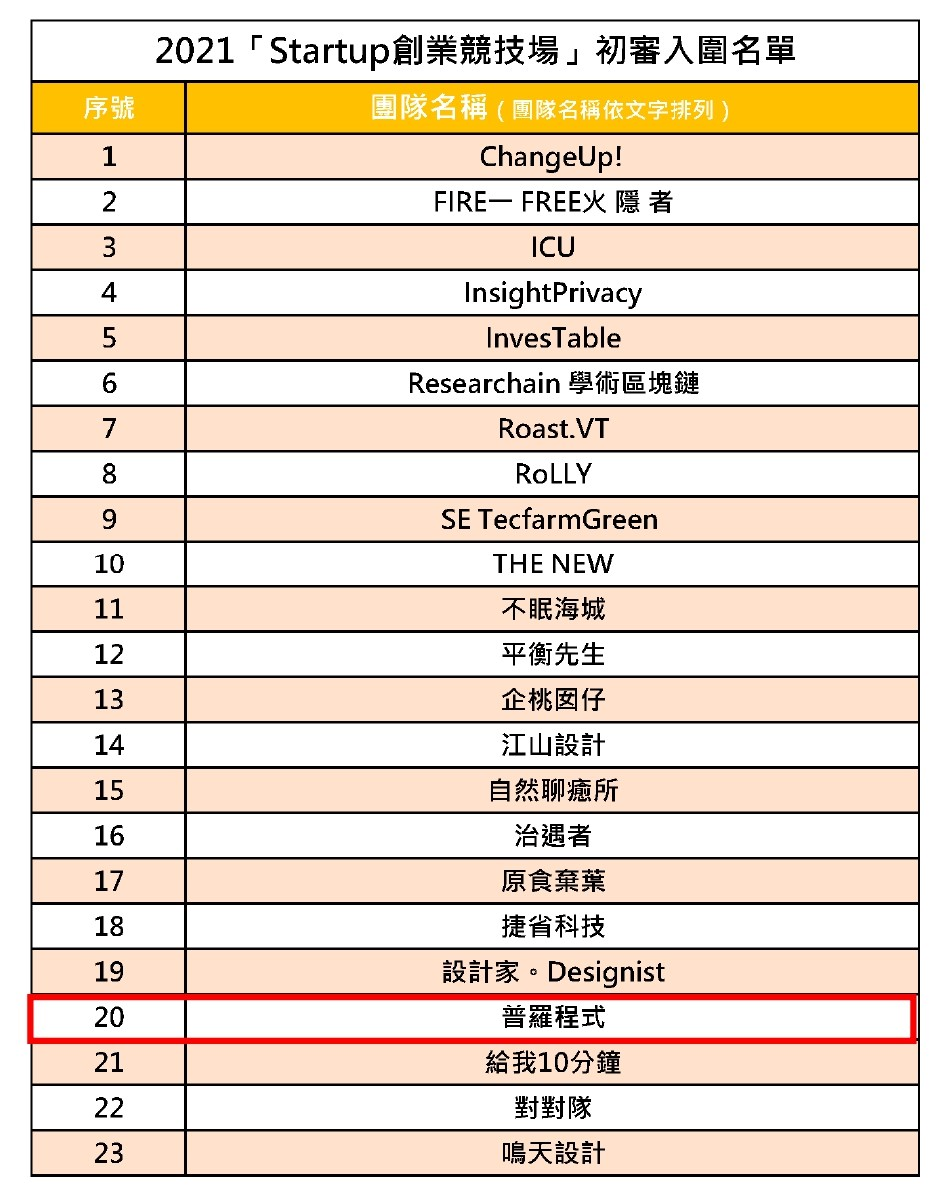
\includegraphics[width=0.6\textwidth]{images/competition-2.jpeg}
		\caption{2021師大Startup競技場決賽}
		\label{fig:Competition-2}
	\end{subfigure}
	\caption{過去的創業競賽經驗}
\end{figure}

% \newpage
% \section{\centering 附件}

% \newpage

\end{document}